\documentclass[tikz,border=2pt]{standalone}
\usepackage{amsmath,amssymb}
\usetikzlibrary{arrows.meta}
\begin{document}
% Two G/G/1 stations in tandem (Exercise 7.1.6): lambda = 2 per hour, C_{a,1}^2 = 2,
% E[S_1] = 1/3 h, E[S_2] = 5/12 h, C_{s,1}^2 = C_{s,2}^2 = 1/2. The departures of station 1 are the
% arrivals of station 2, with C_{a,2}^2 = C_{d,1}^2 ~ 4/3; E[J_1] = 7/6 h and E[J_2] ~ 335/144 h.
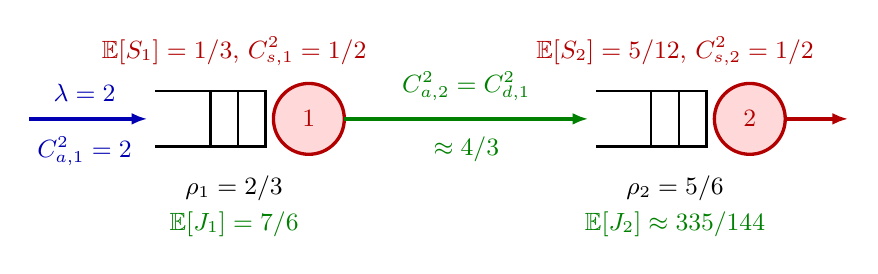
\begin{tikzpicture}[font=\small, >={Latex[length=2mm]}]
  % station 1: queue and server
  \draw[thick] (1.6,0.35) -- (3,0.35) -- (3,-0.35) -- (1.6,-0.35);
  \foreach \x in {2.3,2.65} \draw[thick] (\x,0.35) -- (\x,-0.35);
  \draw[red!70!black, very thick, fill=red!15] (3.55,0) circle (0.45);
  \node[red!70!black] at (3.55,0) {$1$};
  % station 2
  \draw[thick] (7.2,0.35) -- (8.6,0.35) -- (8.6,-0.35) -- (7.2,-0.35);
  \foreach \x in {7.9,8.25} \draw[thick] (\x,0.35) -- (\x,-0.35);
  \draw[red!70!black, very thick, fill=red!15] (9.15,0) circle (0.45);
  \node[red!70!black] at (9.15,0) {$2$};
  % flows
  \draw[->, blue!70!black, very thick] (0,0) -- (1.5,0);
  \node[blue!70!black, anchor=south] at (0.7,0.1) {$\lambda=2$};
  \node[blue!70!black, anchor=north] at (0.7,-0.1) {$C_{a,1}^2=2$};
  \draw[->, very thick, green!50!black] (4,0) -- (7.1,0);
  \node[green!50!black, anchor=south] at (5.55,0.1) {$C_{a,2}^2=C_{d,1}^2$};
  \node[green!50!black, anchor=north] at (5.55,-0.1) {$\approx 4/3$};
  \draw[->, very thick, red!70!black] (9.6,0) -- (10.4,0);
  % station data
  \node[red!70!black, anchor=south] at (2.6,0.55) {$\mathbb{E}[S_1]=1/3$, $C_{s,1}^2=1/2$};
  \node[red!70!black, anchor=south] at (8.2,0.55) {$\mathbb{E}[S_2]=5/12$, $C_{s,2}^2=1/2$};
  \node[anchor=north] at (2.6,-0.6) {$\rho_1=2/3$};
  \node[anchor=north] at (8.2,-0.6) {$\rho_2=5/6$};
  \node[green!50!black, anchor=north] at (2.6,-1.05) {$\mathbb{E}[J_1]=7/6$};
  \node[green!50!black, anchor=north] at (8.2,-1.05) {$\mathbb{E}[J_2]\approx 335/144$};
\end{tikzpicture}
\end{document}
